\documentclass[smallextended]{svjour3}
\usepackage{fix-cm}
\usepackage[T1]{fontenc}
\usepackage[utf8]{inputenc}
\usepackage{mathptmx}
\usepackage{amsmath,amssymb,graphicx,booktabs,tabularx,url}
\usepackage{placeins}
\usepackage[numbers,sort&compress]{natbib}
\usepackage[hidelinks]{hyperref}
\journalname{Computing}
\smartqed
\begin{document}
\title{Selection Resolution, Random-World Coupling, and Utility in Candidate-Restricted Influence Maximization}
\titlerunning{Selection resolution, coupling and utility}
\author{\mbox{Jiayue Sun} \and \mbox{Binbin Yong} \and \mbox{Junjie An} \and \mbox{Tianyu Bo} \and \mbox{Shuai Li}}
\authorrunning{Jiayue Sun et al.}
\institute{Jiayue Sun \at School of Artificial Intelligence, Lanzhou University, Lanzhou 730000, China
\and Binbin Yong (corresponding author) \at School of Information Science and Engineering, Lanzhou University, Lanzhou 730000, China \\
\email{yongbb14@lzu.edu.cn}
\and Junjie An, Tianyu Bo and Shuai Li \at Lanzhou University, Lanzhou, China}
\date{}
\maketitle
\begin{abstract}
Candidate restriction can accelerate greedy influence maximization, but its evaluation depends on the finite simulation reference. We examine selection resolution, random-world coupling, independently evaluated utility and attributable computation cost in a common protocol. An archived experiment on four contact-derived networks is extended by 520 conditions and 4,680 arm executions, using ten random paths per real network, selection budgets up to 5,120 worlds and 10,000 disjoint evaluation worlds. Controls include alternative candidate rankings, propagation parameters, fixed-edge coupling and two synthetic 2,000-node instances. Between 1,280 and 5,120 selection worlds, 16 of 40 full-greedy final sets changed, while average independent spread increased by 0.011 nodes. At the highest budget, weighted-degree 4k pools had network-specific mean spread differences ranging from -0.610 to -0.005 activated nodes relative to full greedy. Topology-degree and PageRank 4k pools reproduced 39/40 and 40/40 ordered references, respectively, showing that weighted-degree losses do not characterize all restrictions. A three-node counterexample shows that step-indexed shared randomness need not produce a monotone finite-world objective, motivating an explicit coupling control. The results separate decision reproduction from utility and expose the dependence of cost-quality interpretations on coverage, ranking and timing scope. The supplied tolerance curves are descriptive; they do not establish practical equivalence, convergence to expected-influence greedy selection or generality beyond the tested simulated settings.
\keywords{influence maximization \and Monte Carlo simulation \and candidate restriction \and reproducibility \and network optimization}
\end{abstract}
\section{Introduction}
Influence maximization selects a small seed set to increase the expected reach of a stochastic diffusion process \cite{ref1}. On a fixed graph, practical implementations must decide both which nodes to consider and how accurately to evaluate them. Candidate restriction reduces the search space, while Monte Carlo sampling approximates spread. These choices interact: a restricted method is often compared with a full-candidate greedy run whose own decisions depend on a finite simulation sample.

An identical seed sequence can establish reproduction of a named computational reference, but cannot by itself establish preservation of expected spread. Conversely, two different sequences can have similar independent utility. This distinction becomes consequential when changing the simulation budget changes the full reference, or when a nominally restricted candidate pool already contains every vertex. A cost comparison is also incomplete unless it specifies whether ranking, world preparation, optimization and evaluation are included.

The broader influence-maximization literature already addresses sampling accuracy, computational efficiency and benchmarking \cite{ref2,ref8,ref9,ref10,ref16}. We therefore do not present sample sensitivity as a new general discovery. Our question is narrower: how should candidate restriction be evaluated when the reference, shared random worlds and practical loss criterion are all implementation choices? We examine membership, independent utility and measured cost together, rather than treating any one as a surrogate for the others.

An initial four-network experiment motivated this study. We preserve that experiment and distinguish it from a prospectively specified extension with additional paths, higher budgets, alternative rankings, propagation parameters and a random-world coupling control. The extension reuses the four observed contact topologies and adds two explicitly synthetic structural instances. It does not supply new observed information cascades or a random sample of real-world networks.

The contribution is an auditable evaluation of this joint decision problem. First, we separate seed-set instability from independently measured utility under nested selection budgets. Second, we examine whether the findings depend on historical contact weights, candidate coverage or random-world coupling. Third, we provide loss-tolerance and cost descriptions with path variability and reproducible records. The implementation is exhaustive per-round greedy enumeration, accelerated without pruning. No new approximation guarantee, universal candidate threshold or learned ranking advantage is claimed.

\section{Related work}
\paragraph{Optimization and sampling.}
The classical formulation relates seed selection to expected diffusion and establishes approximation results under appropriate model assumptions \cite{ref1}. CELF avoids redundant marginal evaluations by exploiting objective structure \cite{ref7}. StaticGreedy reuses sampled realizations to retain the structure of a finite sampled objective \cite{ref8}. IMM uses a different sampling design and algorithm-specific statistical guarantees \cite{ref2}. These methods address computational efficiency and accuracy; their guarantees must not be transferred to a different finite-world implementation without checking its assumptions.

Our reference enumerates every eligible node at every greedy round. It does not enumerate all size-$k$ sets and is not an exact expected-influence optimum. In addition, the original simulator shares random draws by edge and propagation step. This coupling can differ from fixing one live-edge graph per world, even when the marginal diffusion law for a fixed seed set is the intended independent-cascade law. Section~\ref{sec:coupling} makes this implementation distinction explicit and supplies a fixed-edge control.

\paragraph{Candidate selection and learning.}
Candidate sets can be selected using local structure. Published approaches include the neighbour scale fixed method and discrete Harris hawks optimization \cite{ref12,ref13}. Learning-based approaches add training, representation and tuning choices \cite{ref10,ref14}. We compare simple rankings with matched candidate counts to isolate the role of candidate eligibility. This does not rank those published algorithms against each other, and it does not validate a graph neural network selector.

Recent inductive influence estimation, exemplified by MONSTOR+, replaces repeated simulation with learned predictions on unseen graphs under IC and LT models \cite{ref19}. That approach changes the spread estimator. Our controls retain the simulator and vary seed eligibility and reference resolution, addressing a complementary evaluation question without claiming superiority over a trained estimator.

\paragraph{Diffusion and evaluation.}
Temporal influence maximization explicitly models evolving interactions \cite{ref11}; aggregating a historical contact window does not do so. Likewise, observed proximity does not identify an empirical information-influence model \cite{ref15}. Our contact records supply topology only. Benchmarking studies have highlighted the importance of comparable implementations and evaluation settings \cite{ref16}. The associated methodological debate further motivates explicit cost and quality definitions, but we do not adopt disputed algorithm rankings. Table~\ref{tab:position} states the narrower role of the present study.

\begin{table}[t]
\caption{Positioning by the question addressed, rather than by a claim that earlier work omitted every diagnostic.}\label{tab:position}
\begin{tabularx}{\linewidth}{lX}
\toprule
Work or approach & Principal role relative to this study \\
\midrule
Classical greedy \cite{ref1} & Expected-spread formulation and objective-dependent approximation framework \\
CELF \cite{ref7} & Avoiding redundant evaluations when the required objective structure holds \\
StaticGreedy \cite{ref8} & Consistent sampled realizations and scalable optimization \\
IMM \cite{ref2} & A different sampling and guarantee framework \\
Benchmarking \cite{ref16} & Comparative implementation and performance evaluation \\
Present study & Candidate eligibility, reference resolution, coupling, independent utility and attributable costs on a specified matrix \\
\bottomrule
\end{tabularx}
\end{table}

\section{Methods}
\subsection{Task and finite-world reference}
Let $G=(V,E)$ be a directed graph, $k$ the seed budget and $h$ the propagation horizon. A seed is active initially. Each newly activated node has one opportunity to activate each inactive outgoing neighbour with probability $p$, and activation is propagated for at most $h$ rounds. The total spread $f_h(S;\omega)$ includes the seeds. The selection objective for a fixed list of $W$ worlds is
\begin{equation}
\widehat\sigma_{W,h}(S)=\frac{1}{W}\sum_{i=1}^{W}f_h(S;\omega_i).
\end{equation}
Full greedy scans $V\setminus S$ at every round. Restricted greedy scans $C\setminus S$, with a fixed pool $C\subseteq V$. Both choose the largest empirical objective after adding a node and break ties by lexicographic node ID. Nodes outside $C$ remain in the propagation graph.

We denote the ordered trace by $T_W(C)$ and its final set by $S_W(C)$. Ordered agreement, unordered agreement and set Jaccard overlap are reported separately. A pool with $|C|=|V|$ is a full-search consistency control. Its agreement does not demonstrate effective restriction.

\subsection{Random-world coupling and its boundary}\label{sec:coupling}
The original implementation maps a world ID, step and directed endpoint codes to a reproducible 53-bit uniform variate using fixed 64-bit mixing operations. We call this \emph{step coupling}. The same key always supplies the same value, regardless of candidate pool or execution order. Smaller selection budgets are prefixes of larger budgets. This construction is a reproducible pseudorandom scheme, not a proof of independence of all hash outputs.

Step coupling does not imply that each fixed-world objective is monotone. Consider the directed chain $a\rightarrow b\rightarrow c$ with two propagation rounds. Suppose $a\rightarrow b$ is open at step zero, $b\rightarrow c$ is closed at step zero and open at step one. Starting from $\{a\}$ reaches all three nodes, whereas starting from $\{a,b\}$ reaches only two: $b$ attempts transmission earlier. Thus, for this world,
\begin{equation}
\{a\}\subset\{a,b\},\qquad f_2(\{a\};\omega)=3>2=f_2(\{a,b\};\omega).
\end{equation}
The archived hash realizes this example at world ID 5, $p=0.5$ and endpoint codes $0,1,2$. This is a finite-objective counterexample, not evidence that the intended IC marginal distribution is incorrect. It prevents importing a monotonicity or submodularity guarantee into this sampled objective without further work.

Our \emph{fixed-edge coupling} control uses the step-zero variate for each edge throughout a world. Spread then equals the union of nodes reachable within $h$ live-edge hops from each seed, a coverage objective. With independent edge draws, both couplings implement the same finite-horizon IC marginal law for a fixed $S$, but couple different seed sets differently. The empirical comparison keeps the coupling label explicit. Both implementations use full enumeration; no lazy-forward assumption is needed.

\subsection{Independent utility and path uncertainty}
For selected sets, a separate evaluation stream $\mathcal E$ gives the paired difference
\begin{equation}
\widehat\Delta_W(C)=\frac{1}{M}\sum_{i=1}^{M}
\left[f_h(S_W(C);\eta_i)-f_h(S_W(V);\eta_i)\right].
\end{equation}
The same evaluation worlds are shared across arms and selection budgets within each network/path. We retain all per-world counts. The paired Monte Carlo standard error is $s_d/\sqrt M$, conditional on the chosen sets, graph and simulator. Identical sets have identically zero paired differences. These conditional intervals do not measure selection-path variability.

We also report incremental spread $\widehat\sigma-k$. Relative incremental loss is $-\widehat\Delta/(\widehat\sigma_{\rm full}-k)$ when the denominator is positive. Total-spread normalization alone can obscure a loss relative to the additional activations generated beyond the seeds. We do not assign an acceptable loss for a real application. We describe paths at six illustrative loss thresholds: 0, 1, 2.5, 5, 10 and 20 percent. These descriptions do not constitute equivalence or noninferiority tests.

For each fixed network and setting, the extension reports means, sample standard deviations and percentile bootstrap intervals from 10,000 resamples of the path-level observations. The ten paths are computational replicates, not independent networks. The three random pools are averaged within each path before these summaries. Conditional MC intervals and across-path bootstrap intervals are labelled separately; ten paths give limited precision for tail behaviour.

The prespecified primary testing family contains six candidate types versus full greedy on four real networks at $k=5,W=5120,p=0.01,h=3$ under step coupling. We use two-sided exact sign tests for positive/negative balance across paths, drop and report exact zeros, and apply Holm correction over all 24 contrasts. These tests concern the direction of conditional path differences, not a test of a mean effect or a population of networks. All contrasts and effect sizes are provided, including nonsignificant ones.

\subsection{Implementation and timing}
The new engine compiles exhaustive simulations on compressed sparse row graphs with Numba. It preserves the archived hash and tie policy. Integer total spread determines candidate order; at the tested $W\leq5120$, the smallest nonzero mean difference exceeds $10^{-6}$, so this agrees with the archived micro-unit rounding. Audit tests compare the original Python simulator with the new implementation and compare fixed-edge outcomes with an independent shortest-path oracle.

World states are materialized once per condition and shared by all arms. We separately record graph preparation, ranking, shared world preparation, selection and evaluation. Selection-time savings describe an online scenario with prepared graph and worlds. The attributed full-pipeline cost charges each arm the common graph/world preparation plus its own ranking, selection and evaluation. This attribution describes a standalone use of an arm; it is not the elapsed time of executing all arms together.

Arms execute serially in a deterministic randomized order. Five additional randomized timing repetitions per real graph use $k=5,W=320$, path 1001 and the primary propagation setting. Compilation is warmed and excluded from these timings, with compilation overhead recorded separately. The original Python timings and new compiled timings are not pooled or used as an algorithmic speed comparison.

\section{Experimental design}
\subsection{Observed topologies and synthetic controls}
The observed topologies derive from the 2013 and 2015 InVS workplace contacts, SFHH 2009 conference contacts and 2012 Kenyan household contacts \cite{ref3,ref4,ref5,ref6}. Each undirected event becomes two directed events. The first 65\% of complete timestamp groups are retained, self-loops are removed and repeated endpoints collapse for diffusion. Historical outgoing event counts determine weighted degree; because contacts are bidirectional, this ranks incident contact frequency. Diffusion uses a uniform edge probability rather than contact-frequency probabilities.

The resulting graphs have 91, 212, 402 and 75 vertices, respectively. Their directed edge counts are 1,238, 6,938, 11,856 and 1,044. They contain observed contacts, not observed information cascades. The unused later contacts are not a held-out cascade test set.

Two synthetic graphs have 2,000 nodes each. One uses preferential attachment with parameter 3 and follows the model of Barabasi and Albert \cite{ref17}. The other is a stochastic block model \cite{ref18}. It has four equal blocks of 500 nodes, with edge probabilities of 0.012 within a block and 0.0005 across blocks. The random seed is 20261015 for both. We convert each undirected edge to two directed edges. These are fixed synthetic instances, not empirical datasets. Their event weights are unity, so weighted and unweighted degree coincide by construction.

\subsection{Historical evidence and prospective extension}
The original frozen experiment contained 42 conditions and 168 arm executions: seven network/$k$ settings, two paths, three nested budgets and four arms. The two path IDs were 301 and 302, $W\in\{20,80,320\}$, $p=0.01$, $h=3$, and $M=2000$. That experiment is retained as historical evidence. Final-set and conditional-uncertainty diagnostics were added after its outcomes were inspected.

The extension protocol was frozen after reviewing the original study and running outcome-blind resource timings. It is therefore a prospective computational extension on known networks, not a preregistered replication on unseen datasets. Ten new path IDs, 1001--1010, are used for the real networks, and the first five for each synthetic instance. Evaluation uses $M=10,000$ disjoint worlds per path. Selection/evaluation namespaces, prefixes and 907,200 distinct used or reserved world IDs were checked before execution for collisions.

\begin{table}[t]
\caption{Prospectively specified extension. All arms share each condition. The rows define 520 unique conditions.}\label{tab:matrix}
\begin{tabularx}{\linewidth}{lXr}
\toprule
Component & Settings & Conditions \\
\midrule
Resolution & Four real graphs; $k=5$; ten paths; $W=20,80,320,1280,5120$ & 200 \\
Seed budget & InVS 2013/2015 and Kenya; $k=20$; ten paths; $W=320,1280$ & 60 \\
Parameters & Four real graphs; $k=5,W=320$; ten paths; $(p,h)=(.005,3),(.05,3),(.01,1),(.01,5)$ & 160 \\
Coupling & Four real graphs; fixed-edge coupling; $k=5$; ten paths; $W=320,1280$ & 80 \\
Scale/structure & Two synthetic graphs; $k=5$; five paths; $W=80,320$ & 20 \\
\bottomrule
\end{tabularx}
\end{table}

Unless varied in Table~\ref{tab:matrix}, settings are $p=0.01,h=3$ and step coupling. Each condition includes full greedy, weighted-degree $2k/4k/8k$, unweighted topology-degree $4k$, unweighted PageRank $4k$, and three random $4k$ pools. Pool sizes are capped at $|V|$. Random pool identities are independently generated by repeat within network/path and held fixed across budgets and propagation settings. PageRank uses the unweighted directed topology and the implementation's standard damping parameter 0.85. No selector is tuned on the evaluation outcomes.

\section{Results}
\subsection{Implementation validation and evidence continuity}
All 42 archived output hashes matched the historical validation ledger. The accelerated engine reproduced 32 archived arm traces and all 64,000 corresponding per-world evaluation values exactly. Boundary checks covered empty seed sets, zero and unit transmission probability, and horizons zero through three. Additional cyclic-graph checks matched the original simulator, while fixed-edge results matched an independent shortest-path reachability oracle. These checks support semantic continuity rather than a new algorithm claim.

The original experiment changed all 14 full-greedy final sets at each adjacent transition, 20 to 80 and 80 to 320 worlds. Its weighted $2k$, $4k$ and $8k$ pools matched 0/42, 12/42 and 18/42 ordered traces; after excluding full-pool controls, the respective counts were 0/42, 6/36 and 6/30. These historical counts are not combined with new paths as independent replications.

The extension completed all 520 specified conditions and 4,680 arm executions, retaining 46,800,000 evaluation counts. Source and result hashes, per-round greedy choices, full-pool consistency and paired statistics passed the independent output validator. Total serial execution lasted 32.7 minutes; the recorded peak process working set was 780 MiB. The machine had 20 physical CPU cores and approximately 32 GiB RAM, but experiment computation used one worker. Python 3.13.0, NumPy 2.3.3 and Numba 0.68.0 were used.

\subsection{Membership and utility under higher selection resolution}
At the 20 to 80 transition, 40/40 final sets changed; mean Jaccard overlap was 0.276. At the 80 to 320 transition, 37/40 final sets changed; mean Jaccard overlap was 0.400. At the 320 to 1,280 transition, 34/40 final sets changed; mean Jaccard overlap was 0.586. At the 1,280 to 5,120 transition, 16/40 final sets changed; mean Jaccard overlap was 0.789. These summaries describe forty network/path blocks, not forty independently collected networks. Figure~\ref{fig:reference} juxtaposes membership changes with independently evaluated incremental spread.


\begin{table}[t]
\caption{Full-reference utility and final membership. Incremental spread averages ten paths. Last-column differences compare 5,120 with 1,280 worlds on paired independent evaluations; small means are not equivalence tests.}\label{tab:reference}
\centering
\begin{tabular}{lrrrr}
\toprule
Network & Inc. $W=20$ & Inc. $W=5120$ & Same set & Last $\Delta$ \\
\midrule
invs2013 & 1.126 & 1.566 & 9/10 & 0.005 \\
invs2015 & 3.641 & 4.552 & 5/10 & 0.025 \\
kenya2012 & 0.942 & 1.146 & 0/10 & 0.015 \\
sfhh2009 & 7.789 & 8.888 & 10/10 & 0.000 \\
\bottomrule
\end{tabular}
\end{table}
The last two budgets therefore provide a direct check on the practical interpretation of changed membership. Membership changes and small average utility changes do not resolve whether greedy selection has converged for the expected objective. Individual path differences and conditional Monte Carlo intervals are retained in the source tables described in Online Resource 1.
Across these forty blocks, the last transition increased independent spread by 0.0111 nodes on average. Kenya changed all ten final sets whereas SFHH changed none. Thus the remaining membership instability was strongly network-dependent and did not imply a comparably large mean utility change.

\begin{figure}[htbp]
\centering
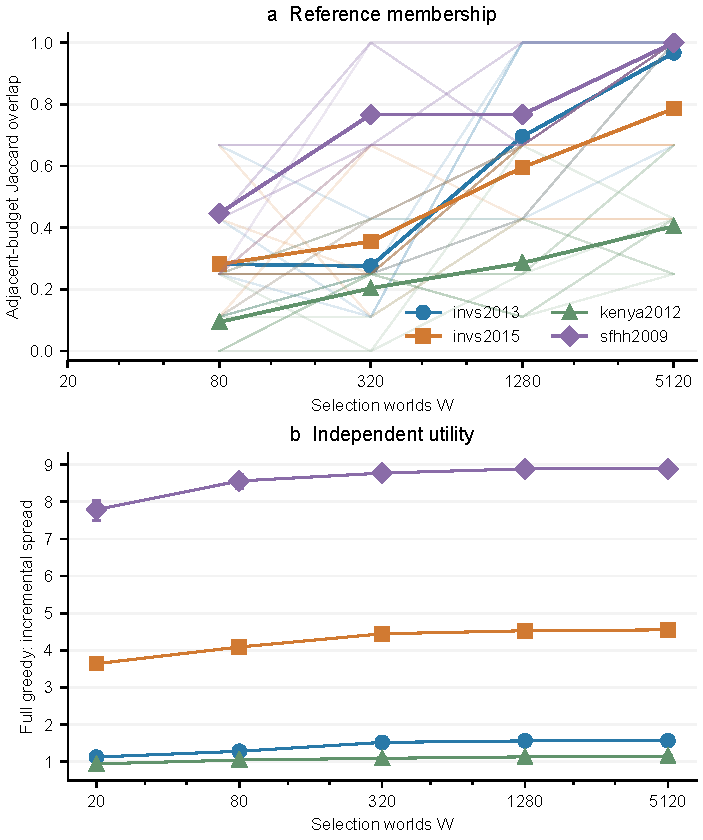
\includegraphics[width=\linewidth]{Fig1.pdf}
\caption{Reference membership and independent utility on four real networks ($k=5$, $p=0.01$, $h=3$, step coupling). (a) Thin lines show all ten path trajectories per network; thick lines show mean adjacent-budget Jaccard overlap. (b) Mean full-greedy incremental spread with 95\% percentile bootstrap intervals over ten paths. Evaluation uses 10,000 disjoint worlds per path. Intervals concern computational paths on fixed graphs; they are not population-network intervals. Colours and marker shapes identify networks}\label{fig:reference}
\end{figure}
\subsection{Candidate rankings and practical loss}
At $W=5120$, weighted-degree $4k$ pools had the following mean paired spread differences (candidate minus full): invs2013: -0.064, invs2015: -0.202, kenya2012: -0.005, sfhh2009: -0.610. Figure~\ref{fig:effects} reports all six candidate types and the across-path intervals, rather than selecting the best pool for each graph.

In contrast, topology-degree and PageRank $4k$ pools reproduced 39/40 and 40/40 ordered full references, respectively. These were genuine restrictions: their twenty eligible nodes represented 5.0--26.7\% of each graph. PageRank therefore had exactly zero paired differences at this setting; degree differed only on one Kenya path, with a slightly higher independently estimated spread. These observations do not establish a universal ranking advantage or future-path equivalence.


\begin{table}[t]
\caption{Mean candidate-minus-full spread changes with reference resolution. W4 and D4 denote weighted-degree and topology-degree $4k$ pools. Each entry averages ten paired path comparisons; signs of means are descriptive, not separate significance claims.}\label{tab:budget-effects}
\centering
\begin{tabular}{lrrrr}
\toprule
Network & W4: 20 & W4: 5120 & D4: 20 & D4: 5120 \\
\midrule
invs2013 & 0.128 & -0.064 & 0.215 & 0.000 \\
invs2015 & 0.364 & -0.202 & 0.539 & 0.000 \\
kenya2012 & 0.126 & -0.005 & 0.127 & 0.001 \\
sfhh2009 & 0.006 & -0.610 & 0.222 & 0.000 \\
\bottomrule
\end{tabular}
\end{table}
Weighted $4k$ had positive mean differences against the low-budget full reference on all four graphs, but negative means against the highest-budget reference (Table~\ref{tab:budget-effects}). The reference quality therefore changes the apparent utility conclusion, not only the trace-match count. Topology degree also gained relative to the low-budget reference, while largely reproducing it at high resolution. This pattern is consistent with a reduced candidate space limiting noisy low-budget choices, but the present contrasts do not isolate that causal mechanism.

In the 24-contrast primary sign-test family, 14 contrasts survived Holm correction at 0.05 (14 with negative and 0 with positive mean differences). The exact tests assess positive/negative balance after dropping zero path differences; they do not test mean equivalence. All unadjusted and adjusted values, zero counts and activated-node effect sizes are supplied in Online Resource 1.

At matched $4k$ coverage, the topology-degree and historical-weighted-degree results can be compared without changing candidate count. Their differences concern the simulator's use of distinct edges rather than event-frequency edge probabilities. Random-pool repetitions are averaged within path and do not triple the inferential sample size.

\begin{figure}[htbp]
\centering
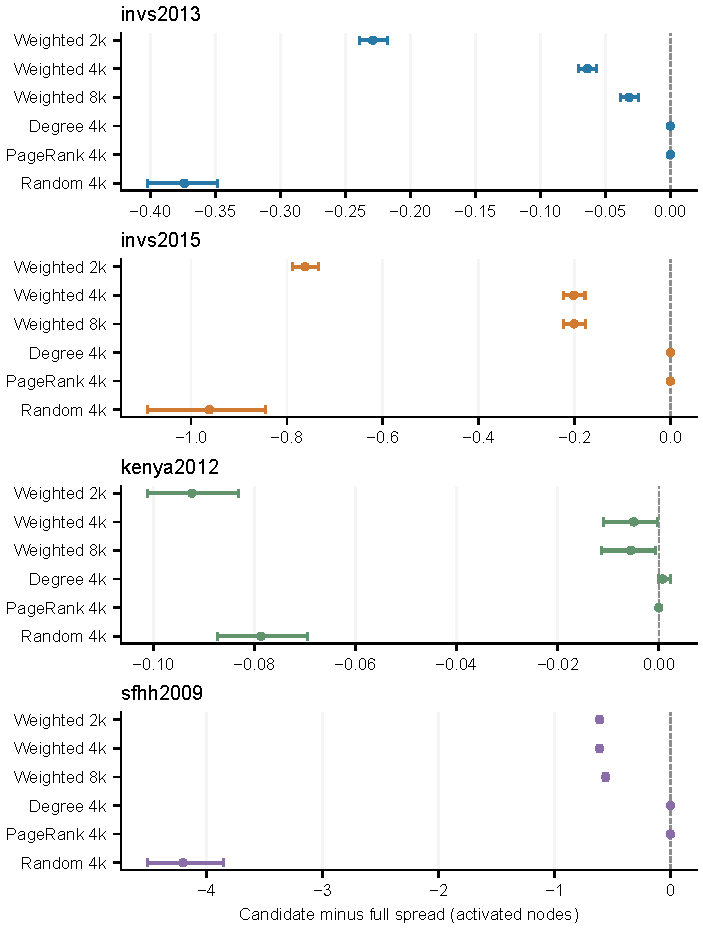
\includegraphics[width=\linewidth]{Fig2.pdf}
\caption{Primary candidate-minus-full spread differences at $W=5120$, $k=5$, $p=0.01$, $h=3$ under step coupling. Points are means of ten path-level differences; horizontal segments are 95\% percentile bootstrap intervals using 10,000 path resamples. Random $4k$ averages three pools within each path. All six candidate types are shown. Horizontal scales differ by network to retain small effects. Zero denotes the full reference, not an equivalence boundary}\label{fig:effects}
\end{figure}
\subsection{Time savings and loss tolerance}
For weighted $4k$ at the primary budget, mean selection-time savings were invs2013: 79.3\%, invs2015: 91.2\%, kenya2012: 74.9\%, sfhh2009: 95.2\%. These percentages exclude shared world preparation. The attributed full-pipeline savings, which include preparation and final evaluation, are reported separately in the source tables.

PageRank $4k$, which reproduced all forty primary references, saved 73.9--94.9\% of selection time across network means; after charging shared preparation and evaluation, savings were 58.0--83.8\%. These are observed cost advantages for this setting, not a guarantee at other budgets or on unseen graphs.

At a loss tolerance of 5\%, the point estimates met the threshold for 10/10 paths on invs2013, 7/10 paths on invs2015, 10/10 paths on kenya2012, 0/10 paths on sfhh2009. This is a description of point estimates at one chosen grid value, not evidence that 5\% is an acceptable application loss or a successful noninferiority test. Figure~\ref{fig:tradeoff} shows the entire prespecified tolerance grid.

\begin{figure}[htbp]
\centering
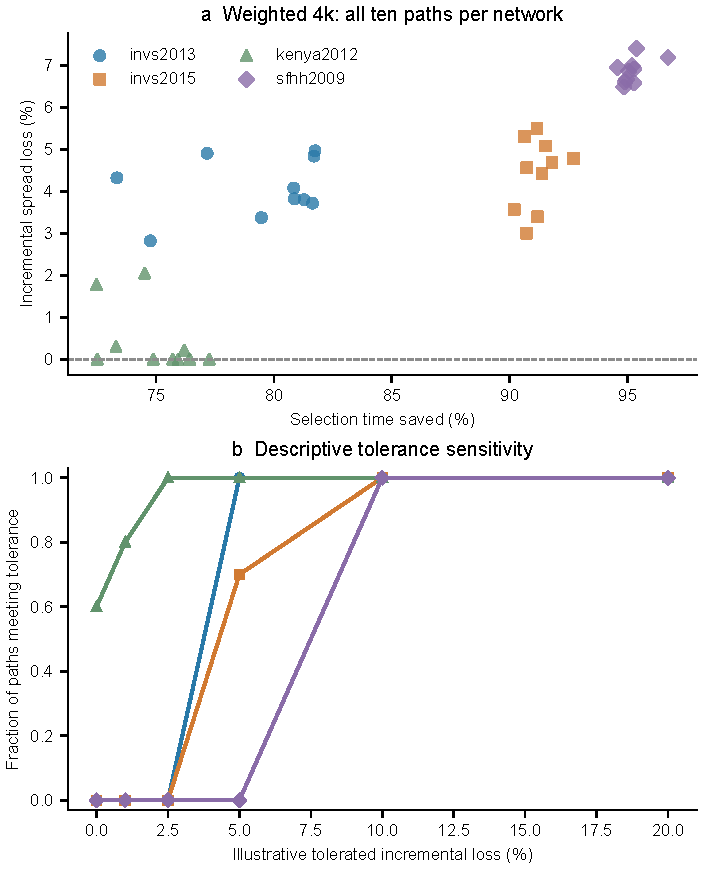
\includegraphics[width=\linewidth]{Fig3.pdf}
\caption{Cost and descriptive tolerance for the prespecified weighted $4k$ diagnostic at $W=5120$. (a) Every one of ten paths per real network is shown; the horizontal axis is selection-only time saving, and the vertical axis is loss relative to full incremental spread. Negative loss denotes a higher candidate estimate. (b) Fraction of paths whose point estimate meets each illustrative tolerance. These are fixed-grid descriptions with a point-estimate denominator, not inferential preservation decisions. All other candidate types remain in the source tables}\label{fig:tradeoff}
\end{figure}
\subsection{Propagation, coupling and structural sensitivity}
The predefined parameter and coupling controls extend the primary setting without changing the candidate rankings. Table~\ref{tab:sensitivity} gives the weighted $4k$ comparison at representative predefined conditions; Figure~\ref{fig:sensitivity} shows all five propagation settings, both couplings and both synthetic instances for its designated panels.

\begin{table}[t]
\caption{Mean weighted $4k$ minus full spread differences. First two columns vary transmission probability at $W=320,h=3$; last two compare couplings at $W=1280,p=0.01,h=3$. Ten paths per cell.}\label{tab:sensitivity}
\centering
\begin{tabular}{lrrrr}
\toprule
Network & $p=.005$ & $p=.05$ & Step & Fixed edge \\
\midrule
invs2013 & 0.004 & -0.513 & -0.065 & -0.061 \\
invs2015 & -0.019 & -1.526 & -0.205 & -0.206 \\
kenya2012 & 0.016 & 0.079 & 0.001 & 0.002 \\
sfhh2009 & -0.228 & -4.983 & -0.630 & -0.616 \\
\bottomrule
\end{tabular}
\end{table}
These contrasts identify sensitivity within the specified grid. They do not establish that one coupling estimates real diffusion more accurately. The two synthetic instances contain 2,000 nodes each, but have only one generated topology of each type. Their five paths measure computational variability on that topology; their agreement cannot substitute for additional real-network evidence. The $k=20$ results similarly retain saturated pools as controls and are tabulated separately.

\begin{figure}[htbp]
\centering
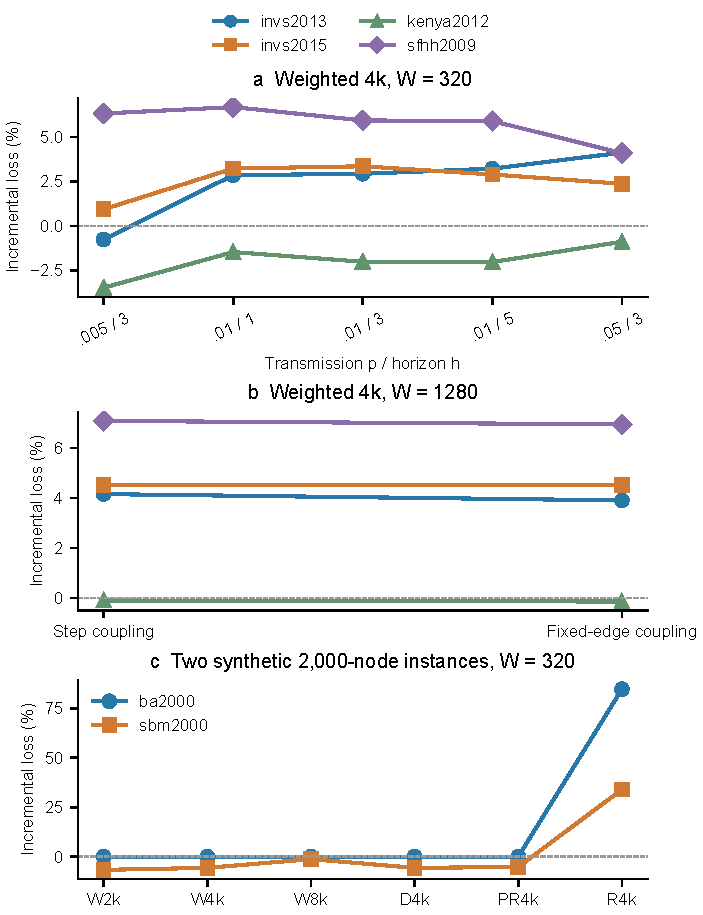
\includegraphics[width=\linewidth]{Fig4.pdf}
\caption{Predefined sensitivity panels. (a) Weighted $4k$ mean incremental loss across ten paths at $W=320$ for all five $(p,h)$ settings, including the primary setting. (b) The same candidate type under step and fixed-edge coupling at $W=1280$. (c) All six candidate types on two explicitly synthetic 2,000-node instances at $W=320$, five paths each; W/D/PR/R denote weighted degree, degree, PageRank and random. Lines connect tested settings without implying interpolation. These panels are descriptive means; all path values and uncertainty summaries are supplied as source data}\label{fig:sensitivity}
\end{figure}
\subsection{Repeated timing}
The five additional repetitions per real graph and arm produced 180 timing observations. Selected sets and all evaluated spreads were unchanged within those repetitions. Figure~\ref{fig:timing} separates selection and evaluation. Repetition measures execution variability in the compiled implementation; it does not increase the number of independent utility observations. Common world preparation and graph preparation remain outside the stacked bars and inside the separately reported full-pipeline attribution.

\begin{figure}[htbp]
\centering
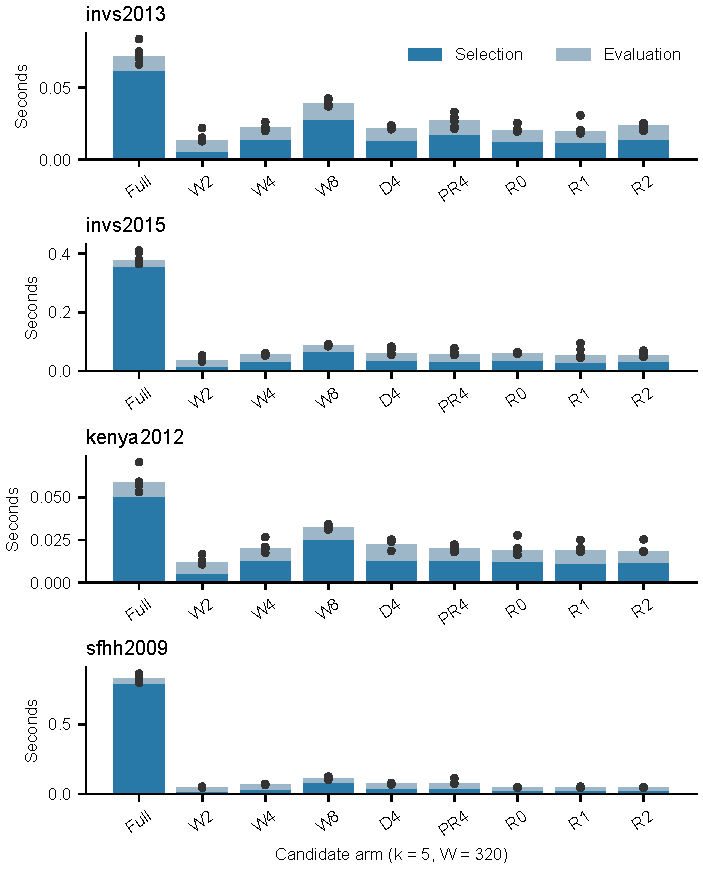
\includegraphics[width=\linewidth]{Fig5.pdf}
\caption{Repeated timing at $k=5,W=320$, path 1001, $p=0.01,h=3$, step coupling. Bars stack the median selection and evaluation times over five additional randomized serial repetitions; dots show each repetition's total of those phases. Full and all eight restricted executions are retained. W2/W4/W8 denote weighted pools; D4 and PR4 denote topology-degree and PageRank; R0--R2 are separate random pools. Shared preprocessing and JIT compilation are excluded from this figure and reported separately}\label{fig:timing}
\end{figure}

\FloatBarrier

\section{Discussion}
The practical interpretation of candidate restriction depends on which quantity is to be preserved. Exact trace reproduction is a statement about a particular finite computation. Independent spread is a property of its selected set under a specified diffusion model. Cost is a property of an implementation and a timing scope. A decision to restrict candidates requires all three to be visible, together with the application's loss tolerance.

Reference instability is therefore a diagnostic rather than a sufficient failure criterion. If selected sets change while independent utility changes little, the algorithm may be moving among similarly useful sets. If utility changes appreciably, a low-resolution reference can alter the apparent quality of a candidate pool. The path-level outputs permit these possibilities to be distinguished instead of interpreting any mismatch as a practically important loss.

The extension narrows the interpretation of the original low-budget findings. Full-reference utility changes diminished at higher budgets even where membership still changed. Weighted-degree pools shifted from positive average differences against the lowest-budget reference to negative differences against the highest-budget reference. At that highest budget, however, topology-degree and PageRank restrictions almost always or always reproduced the full trace. Thus the observed weighted-degree loss cannot characterize candidate restriction in general. The distinction between repeated-contact weights and distinct-neighbour topology is consequential under the uniform-probability simulator.

The coupling audit adds a separate qualification. Consistently reusing random numbers is not by itself a guarantee that the finite objective has the same structure as a fixed-live-edge coverage objective. The explicit chain counterexample isolates this issue without relying on a correlation between ties and changed traces. The fixed-edge control tests sensitivity to the choice; it does not turn the study into a comparison against StaticGreedy or invalidate guarantees proved for that method's own objective.

The ranking result depends on model assumptions. Contact frequency prioritizes repeated encounters. Uniform-probability diffusion on an aggregated graph instead depends on distinct neighbours and their connectivity. Comparing the two degree rankings separates this mismatch from candidate count. It remains a comparison within the simulator, not evidence that contact frequency is generally uninformative in real diffusion.

For reuse, we recommend reporting the actual candidate fraction; the named selection budget and coupling; within-path reference transitions and across-path variability; independent total and incremental spread; and separately attributable costs. A full-pool match should be identified as a control. Any practical preservation claim additionally needs a defensible, prospectively fixed loss criterion and a suitable uncertainty analysis. A large percentage saving is insufficient if the retained incremental spread is unacceptable.

The remaining limitations are material. Four small contact-derived graphs do not represent all social networks. Two synthetic 2,000-node instances establish feasibility at a larger tested size but not web-scale performance or empirical generalization. Transmission probabilities are illustrative and have not been fitted to observed cascades. The grids do not cover all diffusion regimes or learned selectors. Even 5,120 selection worlds do not certify expected-objective convergence. Ten paths limit distributional precision, while the primary sign tests address direction rather than mean superiority. Finally, the code-level acceleration is an implementation tool; the paper's contribution remains the evaluation evidence and its interpretation.

\section{Conclusion}
Evaluating candidate-restricted influence maximization requires a named finite-world reference and an independent utility assessment. The extended protocol separates selection resolution, random-world coupling, candidate ranking and actual coverage, while retaining path-level outcomes and attributable costs. Its findings should be used to characterize conditional trade-offs, not to infer a universal candidate size or to equate trace agreement with utility preservation. The supplied records make these distinctions reproducible within the tested graphs and simulated diffusion settings.
\paragraph{Supplementary information.} Online Resource 1 contains implementation-audit details, the complete primary effect and sign-test tables, round diagnostics, larger-seed-budget summaries and a map to the accompanying reproducibility files.
\section*{Statements and Declarations}
\paragraph{Funding.} This work was supported by a provincial undergraduate innovation and entrepreneurship training project.
\paragraph{Competing interests.} The preceding author draft declares no competing interests.
\paragraph{Author contributions.} The preceding author draft records these roles. Jiayue Sun: conceptualization, methodology, software, validation, analysis, investigation, curation, visualization and original drafting. Binbin Yong: supervision, methodology, project administration, review and editing. Junjie An: software, curation, review and editing. Tianyu Bo: validation, visualization, review and editing. Shuai Li: analysis, validation, review and editing.
\paragraph{Data availability.} The provider records cited above supply the contact data. The accompanying package supplies source references, hashes and preprocessing code; it does not redistribute the provider archives. Synthetic graphs can be regenerated from the documented model parameters and seed. All condition-level results and figure source tables accompany the reproducibility package.
\paragraph{Code availability.} Source snapshots, configuration, validators, analysis and plotting scripts are included in the accompanying reproducibility package.
\paragraph{Use of AI tools.} OpenAI Codex assisted this revision through code development, implementation checks, analysis scripting, figure scripting and manuscript drafting. Verification, scientific interpretation and final approval remain the responsibility of the human authors.
\begin{thebibliography}{16}
\bibitem{ref1} Kempe D, Kleinberg J, Tardos É (2003) Maximizing the spread of influence through a social network. In: ACM SIGKDD, pp 137--146. \url{https://doi.org/10.1145/956750.956769}

\bibitem{ref2} Tang Y, Shi Y, Xiao X (2015) Influence maximization in near-linear time: a martingale approach. In: ACM SIGMOD, pp 1539--1554. \url{https://doi.org/10.1145/2723372.2723734}

\bibitem{ref3} Génois M, Vestergaard CL, Fournet J, Panisson A, Bonmarin I, Barrat A (2015) Data on face-to-face contacts in an office building suggest a low-cost vaccination strategy based on community linkers. Network Science 3:326--347. \url{https://doi.org/10.1017/nws.2015.10}

\bibitem{ref4} Génois M, Barrat A (2018) Can co-location be used as a proxy for face-to-face contacts? EPJ Data Science 7:11. \url{https://doi.org/10.1140/epjds/s13688-018-0140-1}

\bibitem{ref5} Cattuto C, Van den Broeck W, Barrat A, Colizza V, Pinton J-F, Vespignani A (2010) Dynamics of person-to-person interactions from distributed RFID sensor networks. PLoS ONE 5:e11596. \url{https://doi.org/10.1371/journal.pone.0011596}

\bibitem{ref6} Kiti MC, Tizzoni M, Kinyanjui TM, et al. (2016) Quantifying social contacts in a household setting of rural Kenya using wearable proximity sensors. EPJ Data Science 5:21. \url{https://doi.org/10.1140/epjds/s13688-016-0084-2}

\bibitem{ref7} Leskovec J, Krause A, Guestrin C, Faloutsos C, VanBriesen J, Glance N (2007) Cost-effective outbreak detection in networks. In: KDD, pp 420--429. \url{https://doi.org/10.1145/1281192.1281239}

\bibitem{ref8} Cheng S, Shen H, Huang J, Zhang G, Cheng X (2013) StaticGreedy: solving the scalability-accuracy dilemma in influence maximization. In: CIKM, pp 509--518. \url{https://doi.org/10.1145/2505515.2505541}

\bibitem{ref9} Li Y, Fan J, Wang Y, Tan K-L (2018) Influence maximization on social graphs: a survey. IEEE Transactions on Knowledge and Data Engineering 30:1852--1872. \url{https://doi.org/10.1109/TKDE.2018.2807843}

\bibitem{ref10} Li Y, Gao H, Gao Y, Guo J, Wu W (2023) A survey on influence maximization: from an ML-based combinatorial optimization. ACM Transactions on Knowledge Discovery from Data 17(9):1--50. \url{https://doi.org/10.1145/3604559}

\bibitem{ref11} Yanchenko E, Murata T, Holme P (2024) Influence maximization on temporal networks: a review. Applied Network Science 9:16. \url{https://doi.org/10.1007/s41109-024-00625-3}

\bibitem{ref12} Rui X, Yang X, Fan J, Wang Z (2020) A neighbour scale fixed approach for influence maximization in social networks. Computing 102:427--449. \url{https://doi.org/10.1007/s00607-019-00778-5}

\bibitem{ref13} Fan C, Wang Z, Zhang J, Zhao J, Rui X (2024) Influence maximization in social networks based on discrete harris hawks optimization algorithm. Computing 106:327--351. \url{https://doi.org/10.1007/s00607-023-01207-4}

\bibitem{ref14} You K, Liu S, Bai Y (2025) Influence maximization under imbalanced heterogeneous networks via lightweight reinforcement learning with prior knowledge. Complex \& Intelligent Systems 11:40. \url{https://doi.org/10.1007/s40747-024-01666-y}

\bibitem{ref15} Aral S, Dhillon PS (2018) Social influence maximization under empirical influence models. Nature Human Behaviour 2:375--382. \url{https://doi.org/10.1038/s41562-018-0346-z}

\bibitem{ref16} Arora A, Galhotra S, Ranu S (2017) Debunking the myths of influence maximization: an in-depth benchmarking study. In: SIGMOD, pp 651--666. \url{https://doi.org/10.1145/3035918.3035924}

\bibitem{ref17} Barabasi A-L, Albert R (1999) Emergence of scaling in random networks. Science 286:509--512. \url{https://doi.org/10.1126/science.286.5439.509}
\bibitem{ref18} Holland PW, Laskey KB, Leinhardt S (1983) Stochastic blockmodels: first steps. Social Networks 5:109--137. \url{https://doi.org/10.1016/0378-8733(83)90021-7}
\bibitem{ref19} Ko J, Kim S, Lee K, et al. (2025) Inductive influence estimation and maximization over unseen social networks under two diffusion models. Data Mining and Knowledge Discovery 39:55. \url{https://doi.org/10.1007/s10618-025-01137-z}
\end{thebibliography}

\end{document}
